\section{Evaluation}
\label{sec:evaluation}

In this section we present the results of evaluating the energy-saving effects
of using a block-level solution on a SAN environment. There are two
configurations that are compared; the first is the baseline case where a client
machine accesses its back-end storage through an iSCSI connection to a remoter
storage server. In this case, both client and server machines are utilized when
I/O is performed. The client's memory capacity will determine the amount of data
that is cached from the server-side and thus the amount of interactions with the
server. As for the DM-Cache setup, an SSD is used an as additional cache layer
between the client and the server. This layer provides a larger capacity to
cache more data from the server-side, and thus reduce interactions with it. Two
kinds of configurations of DM-Cache are tested; one that caches data from read
operations but sends writes directly to the source device, and one configuration
that caches data from both read and write operations.

\subsection{Experimental Setup}

These tests were performed on two nodes that are part of a Dell 2970
cluster. The source device and the cache device were in separate servers, which
are running Linux 2.6.32 on Ubuntu with 24 GB of RAM.  The initiator (client) is
connected to the target device (source device) using the iSCSI protocol. The
initiator server contained the two disks, an HDD that was used as local storage,
and an SSD that was used as the cache device. The HDD was a 1 TB Seagate
Constellation ES 7200 RPM disk. The SSD cache was a 120 GB Intel SSD 320
Series. The target server (storage server) contained four 1TB HDD with
specifications similar to the one used in the initiator server. One of these was
used for local storage, and another was used as the source device. The remaining
two were not used as part of the tests. For every test DM-Cache was configured
to use a block size of 8 sectors, an associativity of 256, and a cache size of
64 GB. As for the benchmarking tool, IOzone 3.398 and Filebench were used. All
I/O operations were done on a file of size of 8GB or 12GB, and with a request
size of 4 KB.

\subsection{Measuring Power Consumption}

In order to measure the power consumption of a node we used the Watts up? PRO
power meter \cite{wattsup}. This power meter measures the power consumption in
watts with an interval as fast as one second. It came with a USB cable adapter
which we used in combination with an open-source Linux utility tool in order to
download the data directly to a PC.

\subsection{Workloads}

There are several workloads that can receive potential power consumption saving
from using client-side caching. Specifically, clients will benefit more when the
workloads access data that has already been cached to the client-side SSD
device. A system that uses DM-Cache with write-back configuration can support
operations like these. For example, write and read operations which produce hits
on the cache will reduce load on the server-side storage device, and at the same
time reduce the amount of power consumed on the storage server. For the baseline
system setup, a read may be served from the systems page cache, but writes will
always have to be dispatched to the storage server. This results in a constant
use of the server storage device.

Because of the nature of a cache device, we also consider the effect of cache
misses on power consumption. Cache misses caused by operations like a cold read
will inevitably have greater power consumption than the current iSCSI
system. This is because they result in a read operation to read data from the
server storage, and a write operation to write data on the client-side SSD
cache. Thus, workloads that have greater cache hit ratios are the most
appropriate for this type of system.

There are two types of benchmarks that were done in order to cover these cases.
The first consisted of running micro-benchmarks using IOzone. IOzone is a simple
filesystem benchmarking tool that can run a series of simple I/O patterns. For
the purpose of this project we run the sequential reads and sequential writes
operations.  The other kind of benchmarks that were performed were synthetic
workloads using Filebench. Filebench is a benchmarking tool that supports
emulating specific types workloads like fileservers, OLTP systems, web proxies,
and many more workloads. A few of these workloads were run in order to get
insight of the kind of applications that could benefit from the spin-down
daemon.

\subsection{Energy Consumption Results: Micro-Workloads}

\begin{table}
  \centering
  \resizebox{\linewidth}{!}
  {
    \begin{tabular}{|l|l|l|l|l|}
      \hline & \bf iSCSI-W & \bf DMC-WT & \bf DMC-WB-M & \bf DMC-WB-H \\ \hline
      Client & 15589.3     & 16035.6    & 13316.2      & 11664.2      \\ \hline
      Server & 17754.7     & 17874.1    & 14479.4      & 13170.5      \\ \hline
      Total  & 33344       & 33909.7    & 27795.6      & 24834.7      \\ \hline
    \end{tabular}
  }
  \caption{Energy consumption (in Joules) of write operations using an 8GB file}
  \label{tab:write-energy}
\end{table}

\begin{table}
  \centering
  \resizebox{\linewidth}{!}
  {
    \begin{tabular}{|l|l|l|l|}
      \hline & \bf iSCSI-R & \bf DMC-R-M & \bf DMC-R-H \\ \hline
      Client & 13168.8     & 16163.8     & 9119.3      \\ \hline
      Server & 15189       & 18068.1     & 10363.8     \\ \hline
      Total  & 28537.8     & 34231.9     & 19483.1     \\ \hline
    \end{tabular}
  }
  \caption{Energy consumption (in Joules) of read operations using an 8GB file}
  \label{tab:read-energy}
\end{table}


In order to get a general idea of the difference between the power consumption
of I/O requests which are served from the cache device, and those that are
served from the storage server, we performed simple sequential I/O operations
using a tool like IOzone. Table~\ref{tab:write-energy} shows the energy
consumption of both the client and server machines when performing write
requests. The second column (iSCSI-W) shows the energy consumption of writes
performed on with the plain iSCSI system setup. This is the value that we'll use
as a baseline to compare the energy consumption of a system running with
DM-Cache. The next column shows the energy consumption of writes performed on a
system the write-through configuration of DM-Cache (DMC-WT).  Because
write-through operations on DM-Cache are similar to regular iSCSI writes, the
difference between energy consumption of these two is not too much.  The shows
fourth column, a write-back miss (DMC-WB-M), shows energy power consumption of
doing writes on a file that has not been yet cached. Even though this operation
involves cache misses, the energy consumption for this operation is less than
the previous tests, because there are very few reads performed on the server
storage in comparison the number of writes done on the SSD. The last operation
involves writes that produce cache hits. These are the fastest and also the most
energy efficient of all operations.

Table~\ref{tab:read-energy} shows the energy consumption of sequential read
requests. The second columns shows the energy consumed by reads performed on the
system without DM-Cache. The next column shows the results of read misses using
DM-Cache. The results in this particular category show the additional energy
consumed when a read causes a cache miss. The additional energy is caused by the
fact that both the client and server are actively performing I/O, and also
because of the length of the operation. The last column shows the energy saving
potential of client-side caching, as a read hit operation shows a significant
reduction in energy consumption.

Results confirm previous expectations that an SSD cache can help reduce power
consumption. For operations where I/O's are served from the cache device, SSD's
can save up to 25\% energy savings for write operations, and 32\% for read
operations.

\subsection{Micro-Benchmark Analysis}

\begin{figure}[t]
  \centering 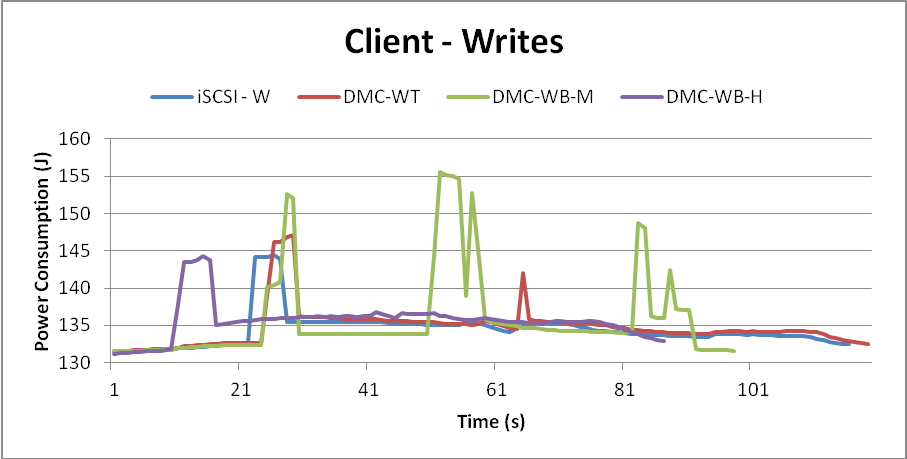
\includegraphics[width=\linewidth]{client_writes.png}
  \caption{Power consumption of write operations on the client}
  \label{fig:client-writes}
\end{figure}

\begin{figure}[t]
  \centering 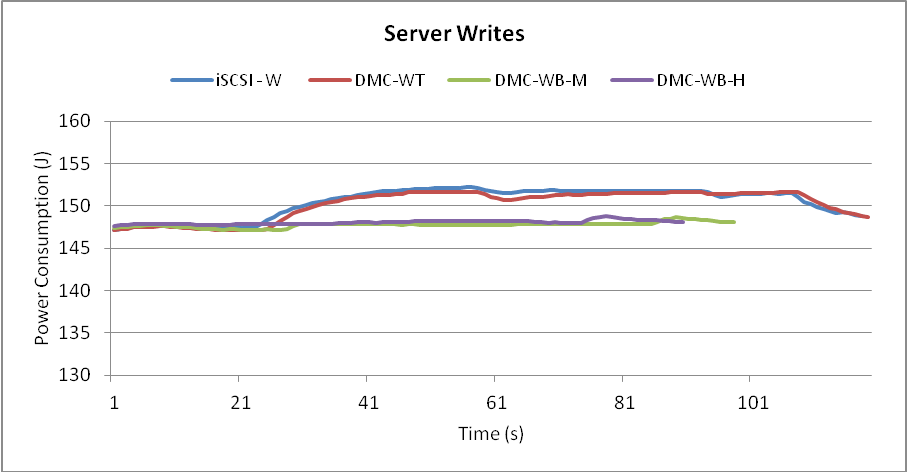
\includegraphics[width=\linewidth]{server_writes.png}
  \caption{Power consumption of write operations on the server}
  \label{fig:server-writes}
\end{figure}

\begin{figure}[t]
  \centering 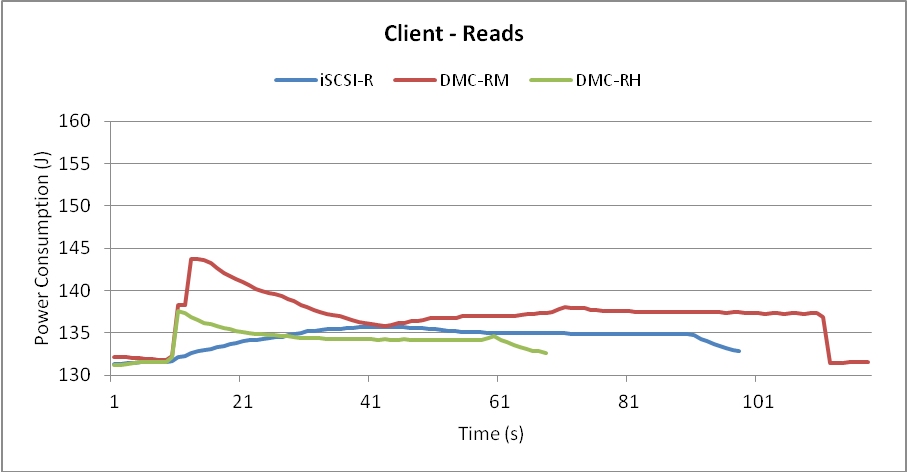
\includegraphics[width=\linewidth]{client_reads.png}
  \caption{Power consumption of read operations on the client}
  \label{fig:client-reads}
\end{figure}

\begin{figure}[t]
  \centering 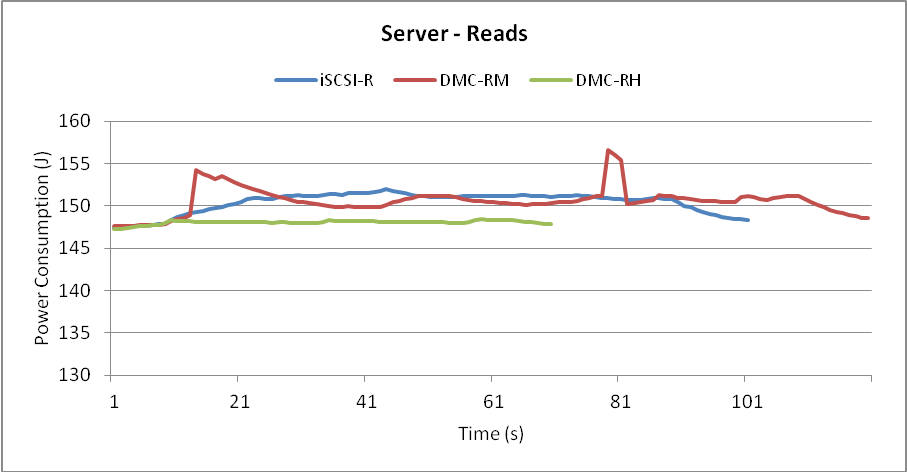
\includegraphics[width=\linewidth]{server_reads.png}
  \caption{Power consumption of read operations on the server}
  \label{fig:server-reads}
\end{figure}

In this section we explore the reasons behind the results of the energy
consumption benefits obtained from an SSD client-side cache device. In order to
this we observe the power consumption graphs yielded by each operation. These
graphs give us several perspectives of the operation ranging from the execution
time of the operation to the power consumption of a specific point in
time. Firstly, let's observe the sequential write operation using the
write-through configuration of DM-Cache. This DM-Cache operation is equivalent
to the regular iSCSI because only reads are served from the cache device, but
write requests are left to be directed to the source device as they normally
would. This means that it is expected that the performance of the iSCSI-W and
the DMC-WT operations be the same or close. Either
Figure~\ref{fig:client-writes} or Figure~\ref{fig:server-writes} can be checked
to confirm that the execution time for these two operations is close, therefore
translating to a similar throughput. A slight increase in power consumption is
seen on the client-side but very little difference on the server-side. The next
test shows the power consumption of DMC-WB-M, which is a write operation that
results in cache misses when performed on the write-back configuration of
DM-Cache. Figure~\ref{fig:client-writes} shows that this operation contains
several spikes of high power consumption on the client-side machine. The reason
for which this operation consumes less energy than an iSCSI-W is that this
operation takes less time to execute and also the power consumption on the
server-side is significantly lower than its corresponding iSCSI-W operation. The
last test is DMC-WB-H, which represents a write operation that results in mostly
cache hits on a write-back configuration of DM-Cache. This operation has a low
power consumption rate on both the client and server-side, and also has a much
faster execution time. This results in the operation that consumes the least
amount of energy.

Figure~\ref{fig:client-reads} and Figure~\ref{fig:server-reads} show the power
consumption of reads on the client and the server side, respectively. The
operation DMC-RM are the reads that are performed on the write-back
configuration of dm-cache that are done on data that is not on the cache device
and result on cache misses. This operation consumes around 18\% more energy than
the iSCSI-R operation. The reason is because a read cache miss triggers a fetch
operation to bring in the data from the source device and another operation to
store this data on the SSD cache device. These additional I/O requests result in
a slower throughput and more energy consumption on both client and server-side,
in comparison to the baseline iSCSI-R operation.  The other read operation,
DMC-RH, shows the power consumption cause by read cache hits. Figure
~\ref{fig:server-reads} shows that initially the power consumption of this
operation on the client-side is similar or slightly higher than the iSCSI-R
operations; however, because of its shorter execution time the operation results
in lower energy consumption. On the server-side power consumption remains low
because the HDD source device remains idle since all read requests are served
from the cache device.

\subsection{Power Consumption: Synthetic Workloads}

\begin{figure}[t]
  \centering 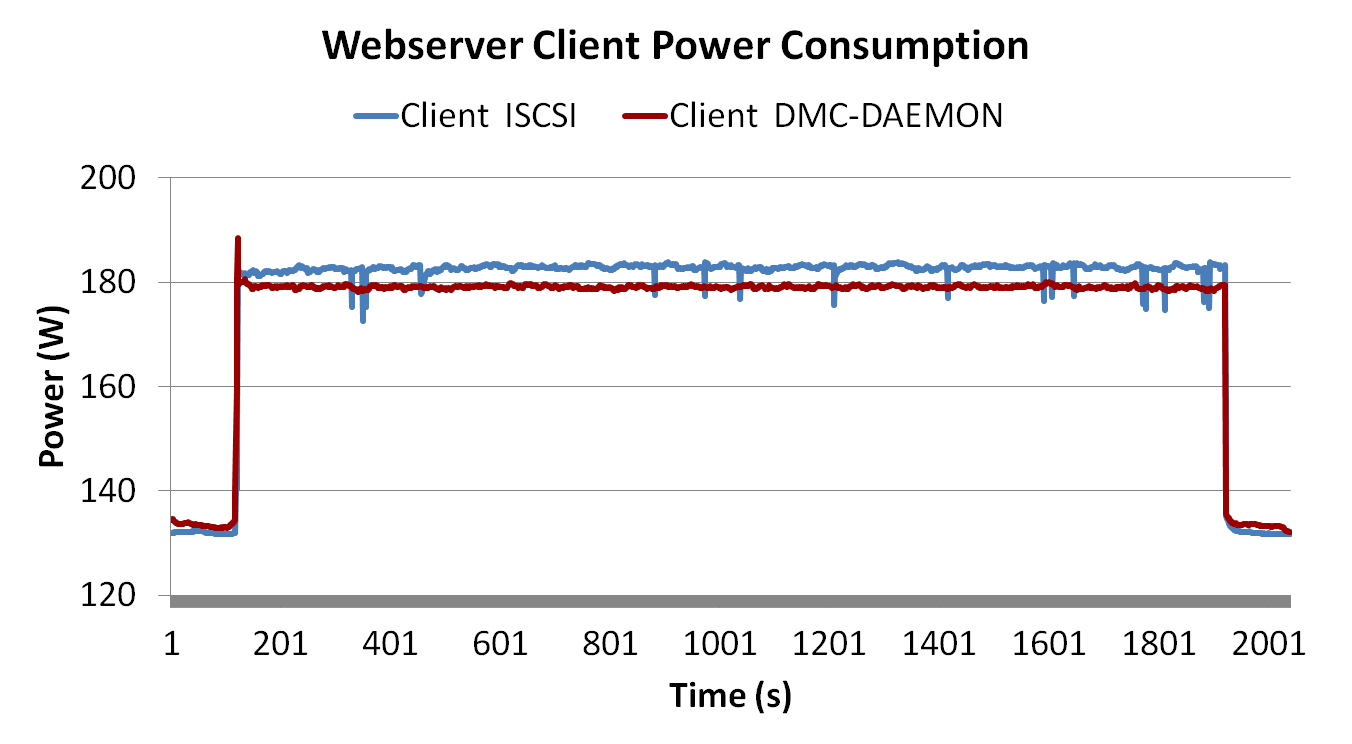
\includegraphics[width=\linewidth]{webserver-client.png}
  \caption{Power consumption of client node of webserver workload}
  \label{fig:webserver-client}
\end{figure}

\begin{figure}[t]
  \centering 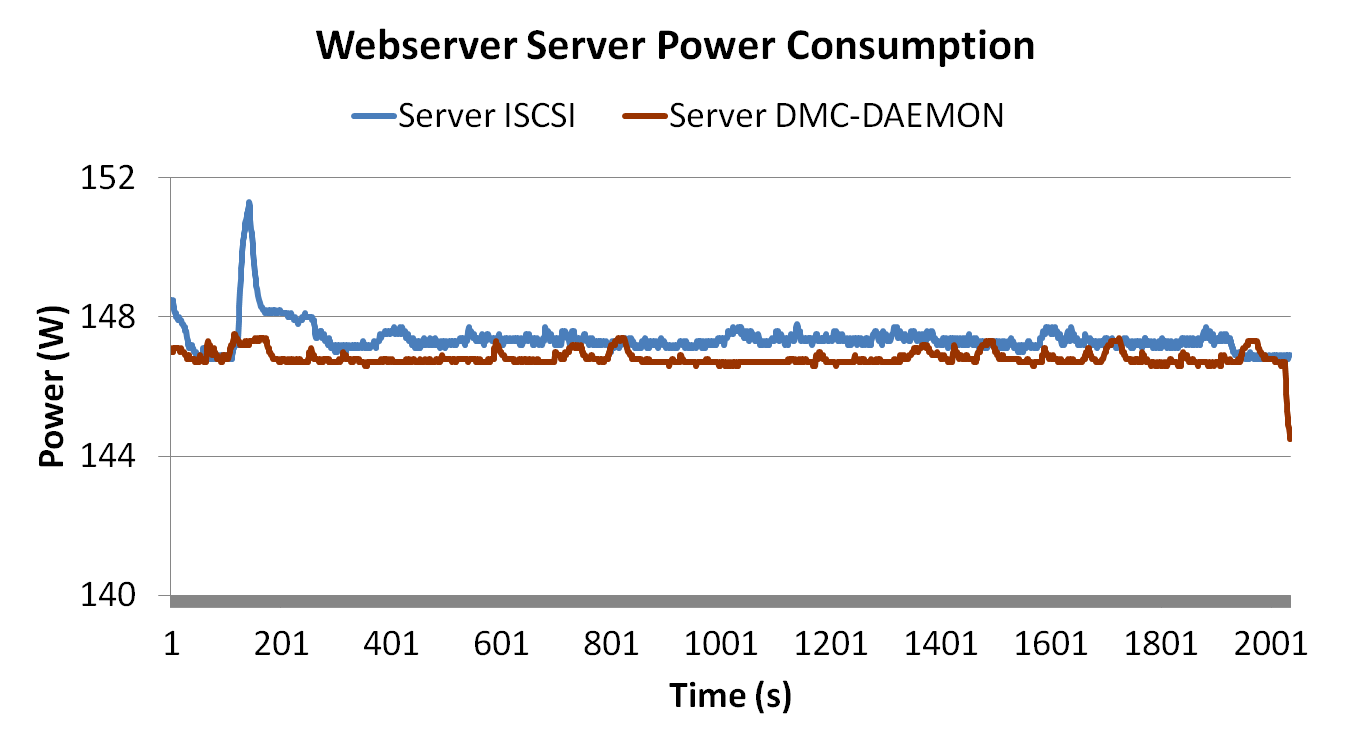
\includegraphics[width=\linewidth]{webserver-server.png}
  \caption{Power consumption of server node of webserver workload}
  \label{fig:webserver-server}
\end{figure}

\begin{figure}[t]
  \centering 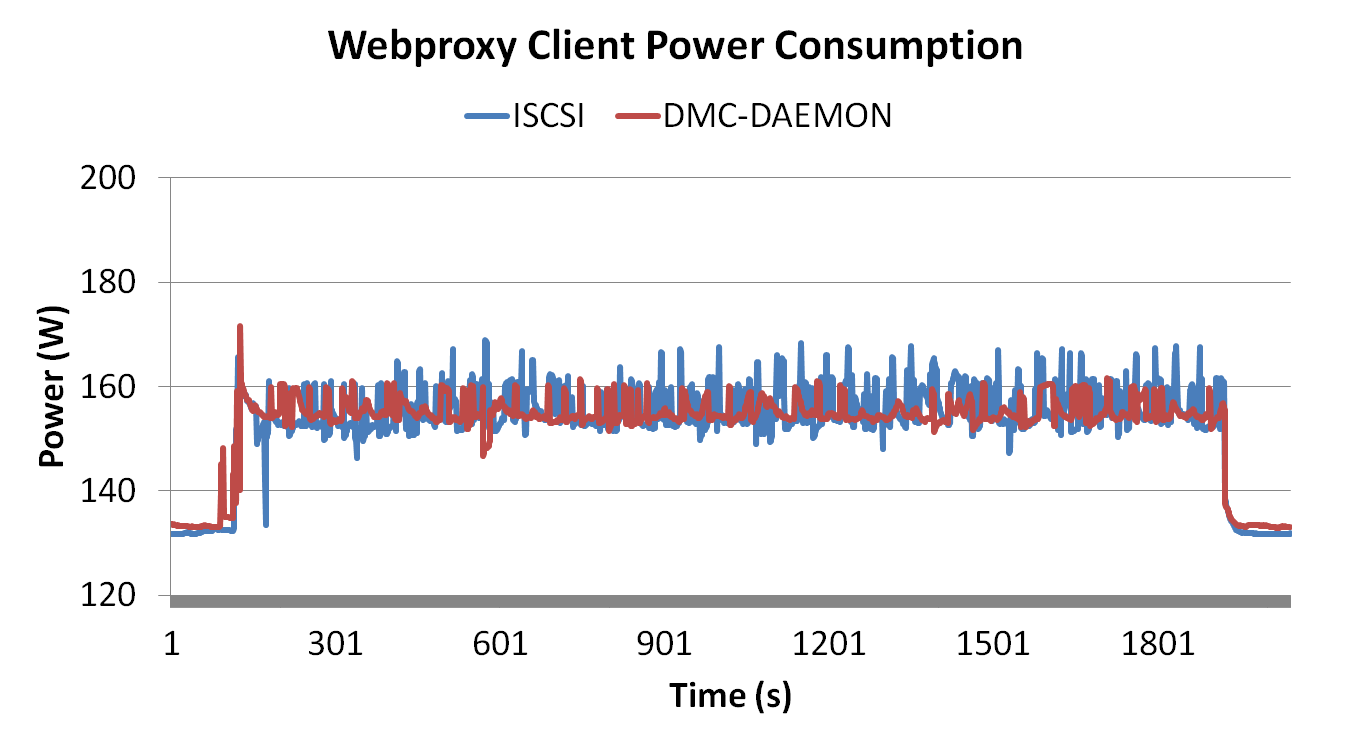
\includegraphics[width=\linewidth]{webproxy-client.png}
  \caption{Power consumption of client node of webproxy workload}
  \label{fig:webproxy-client}
\end{figure}

\begin{figure}[t]
  \centering 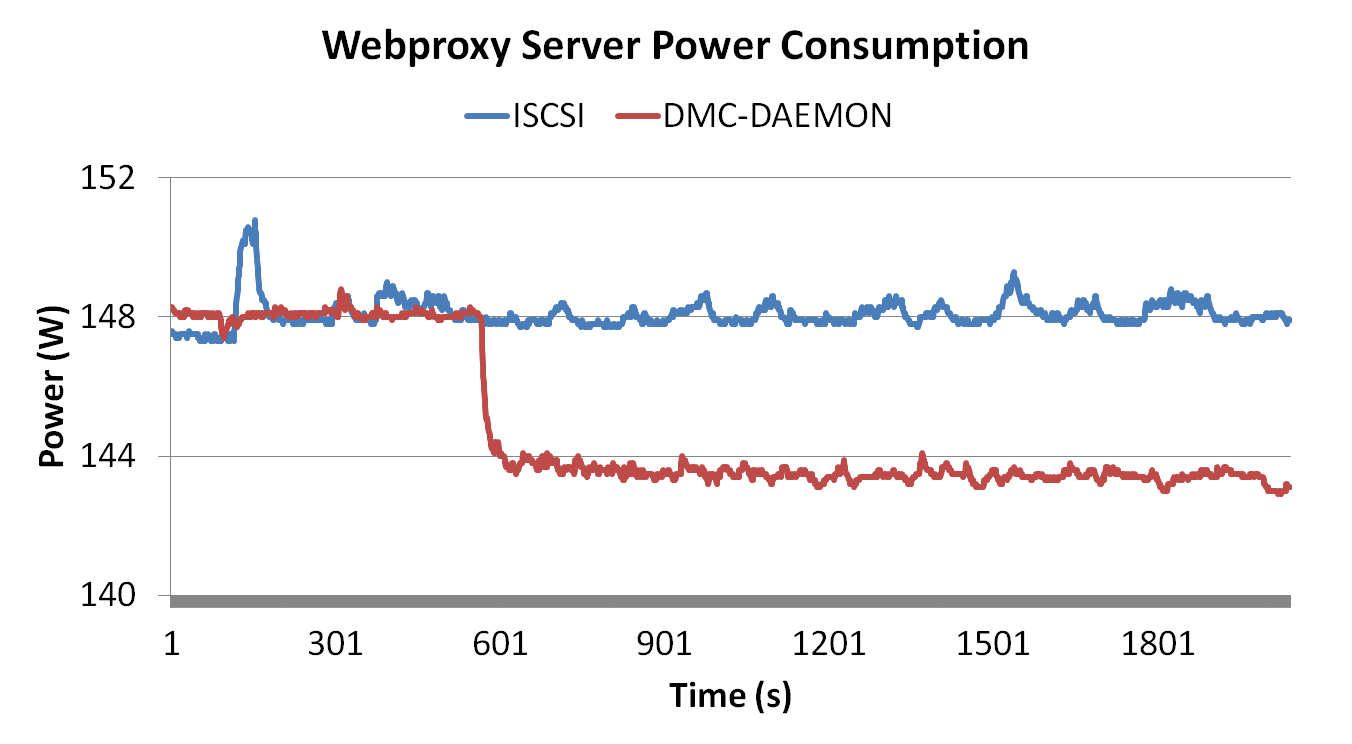
\includegraphics[width=\linewidth]{webproxy-server.png}
  \caption{Power consumption of server node of webproxy workload}
  \label{fig:webproxy-server}
\end{figure}

In order to explore the potential impact of the deamon module in dm-cache we ran
synthetic workloads using the benchmarking tool Filebench. These tests consisted
of running different workload personalities that come with the Filebench tool
package. For these tests we evaluated a series of benchmarks, and chose two
workloads.  The first type of workload that was used for the experiments was the
Filebench webserver personality. This workload consists of emulating a simple
webserver by running a series of open-read-close operations on multiple fles in
a data directory and a log directory. This workload was chosen in order to
observe the cost of running the version of dm-cache with the daemon where the
application does not allow any instances to spin down the disk.  This workload
had close to a 0\% cache hit ratio over the duration of the test which lasted
for 30 minutes. Figure~\ref{fig:webserver-client} and
Figure~\ref{fig:webserver-server} show the power consumption of this workloads.

The first observation from these graphs is that the power consumption for both
client and server is very close. In order to explain this behavior, we fist
should observe the composition of the I/O requests dispatched by the
benchmarking tool. During the beginning of the test, the tool writes a number of
files which are used later for read operations. The graph of the server power
consumption graph shows a momentary increase in power consumption for the iSCSI
configuration and very little increase for the DMC-DAE configuration. This
reflects the amount of I/O requests sent to the server for both
configurations. For iSCSI this is a large increase since all the files written
by Filebench are directed to the storage server disk. For DMC-DAE the increase
in power is small because most data for the files are being written to the
client-side SSD cache. In addition, while files were written to their respective
device, the client's OS was also caching these in memory. This means that these
files will be read from memory instead of the cache device or source
device. This results in few I/O requests served by either the SSD cache or
source device. The similar power consumption of both configurations in the
server graph confirms this behavior. The reason why the server disk keeps
spinning in the DMC-DAE configuration is that there are a series of intermittent
cache read misses which result in data having to be fetched from the storage
source device and then to the client's cache device.


The second type of workload used is a webproxy which emulates the I/O activity
of a simple web proxy.  This workload consists series of mixed create, read, and
delete operations done on multiple files in a data and a log directory. This
kind of workload was chosen because it produced a cache hit ratio of around
70\%, which meant that the disk could have a chance chance to spin
down. Figure~\ref{fig:webproxy-client} and Figure~\ref{fig:webproxy-server} show
the power consumption of this workload in comparison the baseline case, after
being run for 30 minutes. The graph of the power consumption of the server shows
how the disk is spun down after a few minutes or running the tests, signaling
that most IO requests are being served from the cache.

The reason why this type of workload allows for the DMC-DAE configuration to
spin down the disk is based on the characteristics of its I/O
requests. Figure~\ref{fig:webproxy-server} shows the amount of I/O activity that
the server handles.  Before time 600, both configurations show very little
activity on the server-side, with the exception of an slight increase for the
iSCSI configuration.  This spike lasts for the time it takes for the benchmark
to write the test data for the files. This only happens for the iSCSI
configuration and not for DMC-DAE because the data is cached on the client SSD
cache. After time 600, the daemon of DMC-DAE triggers a spin down after
detecting that 1 minute has passed since the last cache read miss. As a result,
the server power consumption graph shows a decrease of around 4 watts. The
client power consumption of both configurations is very similar because the
operations that cause the power consumption are read hits which are served from
the memory cache, and not from the SSD cache device or the storage source
device.
